\model{Loud Toys}

\begin{multicols}{2}
\small

\begin{javalst}
public class ToySheep {
    private int volume;

    public ToySheep() {
        this.volume = 3;
    }

    public int getVolume() {
        return volume;
    }

    public void setVolume(int volume) {
        this.volume = volume;
        makeNoise();
    }

    public void makeNoise() {
        System.out.println("Baaa");
    }
}
\end{javalst}

\begin{center}
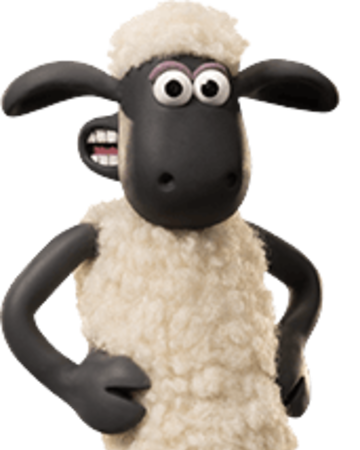
\includegraphics[height=8em]{shaun.png}
\hspace{2em}
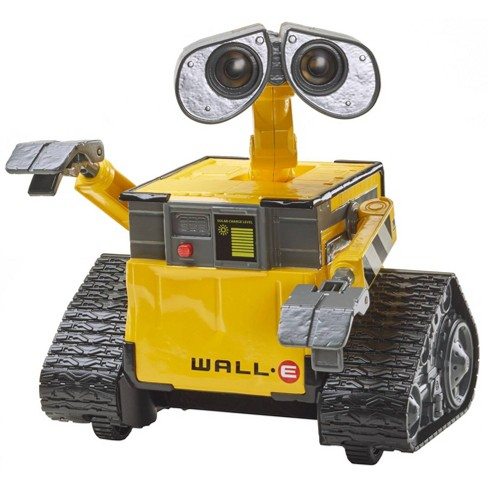
\includegraphics[height=8em]{wall-e.jpg}
\end{center}

\columnbreak

\begin{javalst}
public class ToyRobot {
    private int chargeLevel;
    private int volume;

    public ToyRobot() {
        this.chargeLevel = 5;
        this.volume = 10;
    }

    public void recharge() {
        chargeLevel = 10;
    }

    public int getVolume() {
        return volume;
    }

    public void setVolume(int volume) {
        this.volume = volume;
        makeNoise();
    }

    public void makeNoise() {
        System.out.println("Beep Beep!");
    }
}
\end{javalst}

\end{multicols}


\quest{15 min}


\Q Identify \emph{similarities} in the code:

\begin{enumerate}
\item What attributes do the classes have in common?
\\[1ex] \ans[468pt]{volume}

\item What methods do the classes have in common?
\\[1ex] \ans[468pt]{getVolume, setVolume, makeNoise}
\end{enumerate}


\Q Summarize \emph{differences} between the constructors and the \java{makeNoise} methods.

\begin{answer}
The volume is initialized to 3 in ToySheep, but it's 10 in ToyRobot.
The ToySheep says "Baaa", but the ToyRobot says "Beep Beep!".
\end{answer}


\Q \label{LoudToyV1}
Design a new class named \java{LoudToy} that contains the code that \java{ToySheep} and \java{ToyRobots} have in common.
The constructor of \java{LoudToy} should take \java{volume} as a parameter.
The \java{makeNoise} method should have an empty body.

\begin{javalst}
public class LoudToy {
\end{javalst}
\vspace{-1ex}
\begin{answer}[25em]
\begin{javaans}
    private int volume;

    public LoudToy(int volume) {
        this.volume = volume;
    }

    public int getVolume() {
        return volume;
    }

    public void setVolume(int volume) {
        this.volume = volume;
        makeNoise();
    }

    public void makeNoise() {
        // will be overridden in subclass
    }
\end{javaans}
\end{answer}
\vspace{-1ex}
\begin{javalst}
}
\end{javalst}


\Q Redesign \java{ToySheep} so that it extends \java{LoudToy}.
The constructor of \java{ToySheep} should call the constructor of \java{LoudToy}.
Remove the code from \java{ToySheep} that is no longer necessary.
%Do not duplicate any code in \java{LoudToy}.

\begin{javalst}
public class ToySheep extends LoudToy {
\end{javalst}
\vspace{-1ex}
\begin{answer}[12em]
\begin{javaans}
    public ToySheep() {
        super(3);
    }

    public void makeNoise() {
        System.out.println("Baaa");
    }
\end{javaans}
\end{answer}
\vspace{-1ex}
\begin{javalst}
}
\end{javalst}


\newpage

\Q \label{key1}
Redesign \java{ToyRobot} so that it extends \java{LoudToy}.
Remove the code from \java{ToyRobot} that is no longer necessary.
%Do not duplicate any code in \java{LoudToy}.

\begin{javalst}
public class ToyRobot extends LoudToy {
\end{javalst}
\vspace{-1ex}
\begin{answer}[20em]
\begin{javaans}
    private int chargeLevel;

    public ToyRobot() {
        super(10);
        chargeLevel = 5;
    }

    public void recharge() {
        chargeLevel = 10;
    }

    public void makeNoise() {
        System.out.println("Beep Beep!");
    }
\end{javaans}
\end{answer}
\vspace{-1ex}
\begin{javalst}
}
\end{javalst}


\Q What is the output of the following examples?

\begin{enumerate}

\item
\begin{javalst}
LoudToy toy1 = new LoudToy(1);
toy1.makeNoise();
\end{javalst}

\vspace{-2.5em} \hspace{18em} \ans{(no output)}

\item
\begin{javalst}
LoudToy toy2 = new ToySheep();
toy2.makeNoise();
\end{javalst}

\vspace{-2.5em} \hspace{18em} \ans{Baaa}

\item
\begin{javalst}
LoudToy toy3 = new ToyRobot();
toy3.makeNoise();
\end{javalst}

\vspace{-2.5em} \hspace{18em} \ans{Beep Beep!}

\end{enumerate}


\Q In the previous question, did the variable's type or the object's type determine the version of \java{makeNoise} that was called?

\begin{answer}
The object's type -- notice that the variable type is the same in all three instances.
\end{answer}


%\Q Would it ever make sense to construct a \java{LoudToy} object? Why or why not?
%
%\begin{answer}
%Answers will vary.
%A \java{LoudToy} isn't very useful by itself, since all it can do is get and set volume.
%It needs other attributes and methods to represent an actual toy.
%\end{answer}
